%-*-coding: utf-8-*-

\chapter{Rake-Compress деревья}

Данная глава полностью посвящена Rake-Compress деревьям. 
В ней собрана информация, которую можно найти в опубликованных статьях, необходимая для понимания предложенных в следующей главе оптимизаций.
В главе приведены теоремы, на которых базируются Rake-Compress деревья, 
рассмотрен способ их хранения, 
и показано, как эффективно определить корень дерева, в котором находится заданная вершина, используя Rake-Compress дерево.
Также в данной главе описано, как изменяется Rake-Compress дерево при удалении или добавлении ребер в лес.

\FloatBarrier
\section{Идея}

Входными данными для алгоритма Rake-Compress является лес корневых деревьев. К нему поочередно применяются операции Rake и Compress до тех пор, пока существует хотя бы одна живая вершина. 
Во время каждой из этих операций выбирается некоторое множество попарно несмежных вершин, которое сжимается к своим родителям. 
После каждой операции лес сохраняется в специальном виде, что в дальнейшем дает возможность отвечать на запросы о структуре леса. Рассмотрим более подробно операции Rake и Compress.

Во время операции Rake все листья дерева сжимаются к своим родителям. Пример применения операции Rake показан на рис.~\ref{pic:rake}.

\begin{figure}[h]
\centering
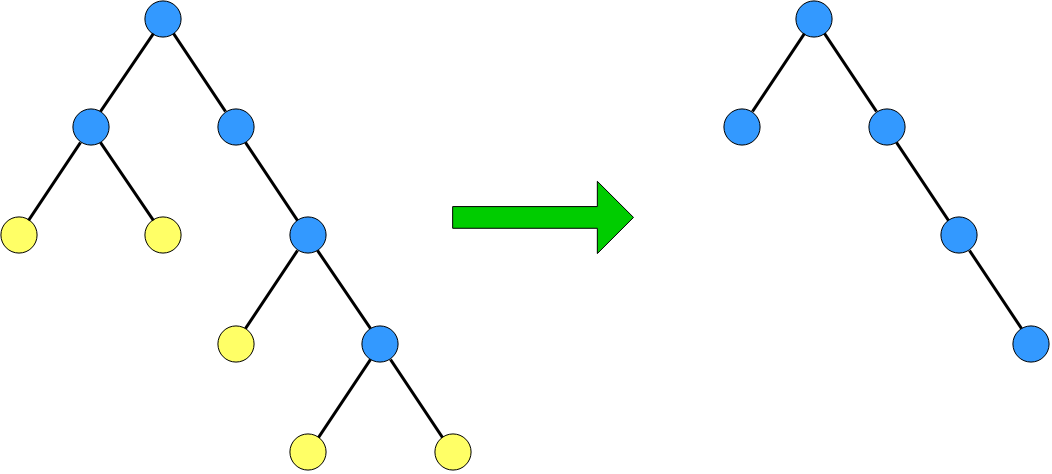
\includegraphics[width=0.8\textwidth]{pics/rake.png}
\caption{Операция Rake}
\label{pic:rake}
\end{figure}

Во время операции Compress выбирается некоторое множество несмежных друг с другом вершин.
Причем каждая такая вершина должна иметь ровно одного сына и при этом не быть корнем дерева. Чтобы выбрать такое множество применяется следующий метод.
Для каждой вершины с помощью генератора псевдослучайных чисел выбирается случайный бит. Вершина добавляется в множество, если у нее:
\begin{itemize}
\item ровно один ребенок;
\item она не является корнем;
\item биты, которые были сгенерированы для нее, ребенка и родителя, равны 0, 1 и 1 соответственно. 
\end{itemize}

Несложно заметить, что в выбранном таким способом множестве не будет смежных вершин.
Пример применения операции Compress показан на рис.~\ref{pic:compress}.

\begin{figure}[h]
\centering
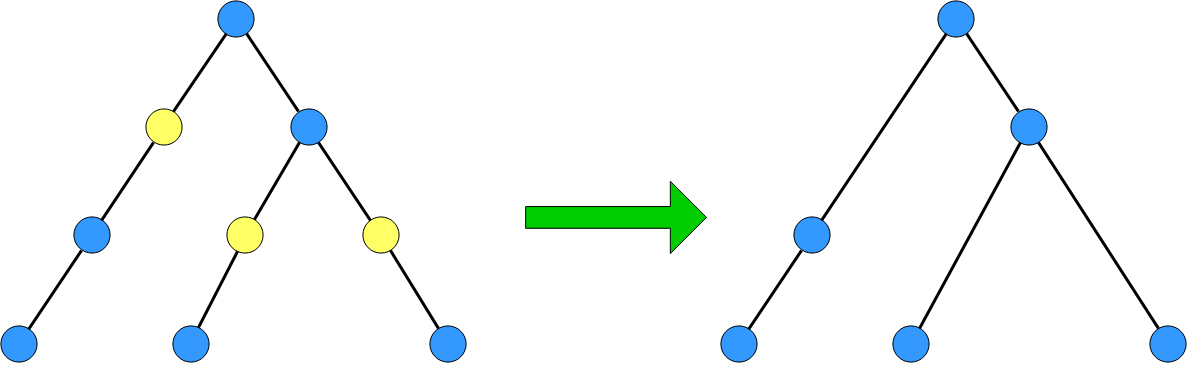
\includegraphics[width=0.8\textwidth]{pics/compress.png}
\caption{Операция Compress}
\label{pic:compress}
\end{figure}

Рассмотрим, как изменяется количество вершин в дереве, после применения к нему операций Rake и Compress. 
Разобьем все вершины дерева на три группы: входящая степень которых равна нулю, одному и больше одного. Обозначим их количество за $T_0$, $T_1$ и $T_2$ соответственно.
\begin{lemma}
\label{lem:cnt_vertices}
  $T_2 \leq T_0 - 1$
\begin{proof}
  Докажем по индукции по высоте дерева. 
  
  Для дерева из одной вершины утверждение верно. 
  
  Пусть утверждение доказано для деревьев высоты меньше $h$. Докажем для дерева высоты ровно $h$. 
  Рассмотрим степень корня. Если корень имеет ровно одного ребенка, то переходим к случаю дерева высоты $h - 1$. Если у дерева несколько поддеревьев, 
  то имеем 
  
  $T_2 = 1 + \sum\nolimits_{u \in children(root)} {T_2 (u)} 
             \leq 1 + \sum\nolimits_{u \in children(root)} {(T_0 (u) - 1)} \\
             \leq -1 + \sum\nolimits_{u \in children(root)} {T_0 (u)} 
             \leq -1 + T_0 = T_0 - 1$. 
  
  Заметим, что для леса деревьев лемма также справедлива.
\end{proof}
\end{lemma}

\begin{lemma}
\label{lem:const_factor}
После применения пары операций Rake и Compress к лесу, математическое ожидание количества вершин в нем не превосходит $\frac{7}{8}$ от их исходного числа.
\begin{proof}
Математическое ожидание количества удаленных вершин $deleted = T_0 + \frac{T_1}{8}$ 
(так как все листья будут удалены после операции Rake, а каждая вершина, у которой ровно один сын, будет удалена с вероятностью $\frac{1}{8}$ после операции Compress). 
Из леммы \ref{lem:cnt_vertices} получаем\\ $deleted = T_0 + \frac{T_1}{8} \geq \frac{1}{2} (T_0 + T_2) + \frac{1}{8} T_1 \geq \frac{1}{8} (T_0 + T_1 + T_2)$
\end{proof}
\end{lemma}
 
\begin{theorem}
\label{the:log}
 Математическое ожидание количества операций Rake и Compress, которые будут выполнены до полного сжатия дерева, равно $O(\log n)$, где $n$ --- общее количество вершин. 
\begin{proof}
Из леммы \ref{lem:const_factor} известно, что после каждой итерации применения операций Rake и Compress число вершин в среднем уменьшается в константное число раз. Значит, количество итераций в среднем ограничено $O(\log n)$.
\end{proof}
\end{theorem}

Из леммы \ref{lem:const_factor} также следует, что математическое ожидание суммарного числа вершин по всем итерациям равно $O(n)$. Это утверждение будет полезно для оценки количества используемой памяти.

\FloatBarrier
\section{Хранение Rake-Compress деревьев}
\label{sec:tree_storage}

Для того чтобы отвечать на запросы относительно структуры леса необходимо сохранить информацию о том, как происходил процесс сжатия леса. 
Будем хранить таблицу, в каждой строке которой будет записано состояние леса после применения операции Rake или Compress.
Каждый столбец таблицы будет соответствовать некоторой вершине. 
А каждая клетка будет хранить состояние некоторой вершины после какой-то итерации. Состоянием вершины будем считать ее родителя, а также множество детей. 
Если же вершина уже была сжата к этому моменту, то пометим это специальным образом. 

Пример такой таблицы показан на рис.~\ref{pic:table}. Рассмотрим более подробно процесс сжатия этого графа. 
Первоначальному состоянию дерева соответствует нижняя строка таблицы. После применения операции Rake к дереву, вершина 4 сжалась к своему родителю --- вершине 3.
Состояние дерева в этот момент сохранено во второй строке снизу. Например, в последнем столбце, который соответствует вершине номер 4, стоит прочерк, так как вершина была сжата к родителю.
После этого к дереву была применена операция Compress и вершина номер 2 сжалась к своему родителю. 
Заметим, что единственная вершина, которая могла быть сжата, во время операции Compress --- вершина номер 2, так как только у нее один ребенок, и она не явлется корнем дерева.
При этом на рисунке изображена ситуация, которая случится с вероятностью $\frac{1}{8}$, а с вероятностью $\frac{7}{8}$ после операции Compress данное дерево не изменится.
После этого произошла операция Rake, и в графе осталась только вершина с номером 1 --- корень дерева. 
Эта вершина будет удалена еще после двух итераций (операция Compress никак не изменит дерево из одной вершины).

\begin{figure}[h]
\centering
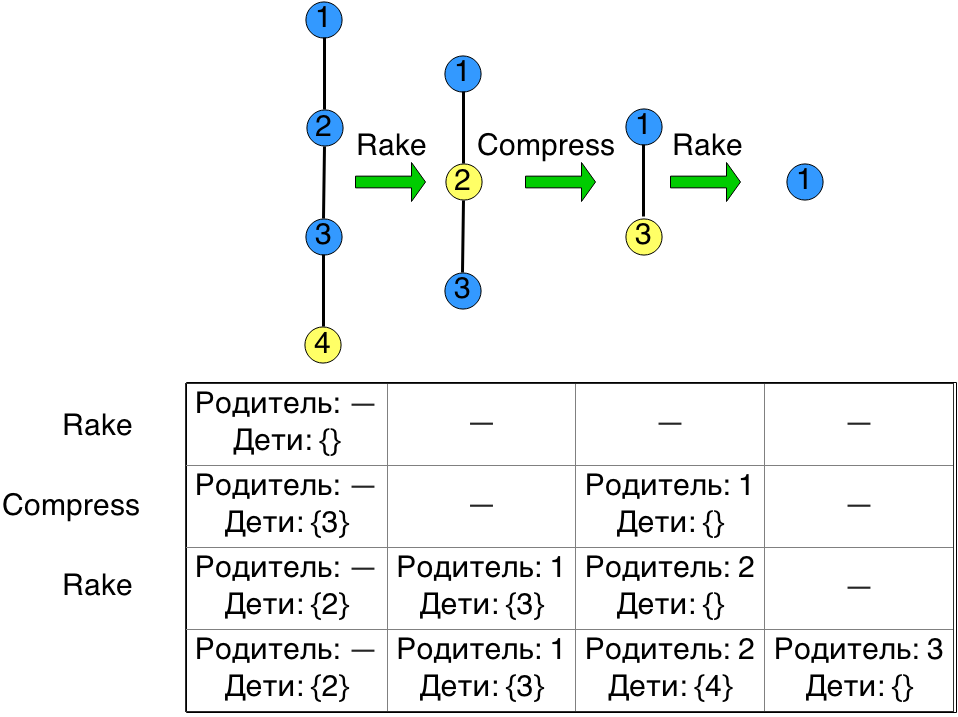
\includegraphics[width=0.8\textwidth]{pics/example.png}
\caption{Хранение Rake-Compress дерева в виде таблицы}
\label{pic:table}
\end{figure}


Из теоремы~\ref{the:log} известно, что математическое ожидание количества строк в такой таблице $O(\log n)$.  
Так как в таблице ровно $n$ столбцов, суммарное количество памяти, которое необходимо для хранение такой таблицы, равно $O(n \log n)$.
Если же в каждой строке хранить только существующие вершины с помощью ассоциативного массива, то количество используемой памяти уменьшится до $O(n)$. 
Однако, на практике использование ассоциативного массива оказывается нецелесообразным из-за большой константы.

\FloatBarrier
\section{Возможность параллельного построения}

Заметим, что операцию Rake и операцию Compress можно выполнять параллельно для всех вершин. 
Единственная часть алгоритма, которую непонятно как реализовать параллельно, является пересчет множества детей вершины при переходе к следующему слою. 
В оригинальной статье степень каждой вершины считалась константой, поэтому множества можно было хранить и пересчитывать любым способом. Если же предположить, 
что множество детей можно пересчитывать за $O(1)$, то Rake-Compress дерево можно построить за $O(\log n)$ в модели PRAM в случае наличия $\Omega(n)$ процессоров.

\FloatBarrier
\section{Ответ на запросы про структуру леса}

Рассмотрим, как с помощью таблицы, которая была описана ранее, отвечать на запросы. Самым простым запросом является ``определить корень дерева, в котором находится вершина $v$''.
Чтобы ответить на этот запрос необходимо проследить за вершиной $v$ в таблице. Будем переходить по строчкам таблицы начиная с первой. Если в некоторой строке нет клетки,
которая соответствует вершине $v$, то необходимо перейти к родителю вершины $v$ на предыдущей строке. Если же у нее не было родителя, то значит вершина $v$ является корнем.

Чтобы проверить, находятся, ли две вершины в одном дереве, необходимо найти корни деревьев, в которых находятся обе вершин и сравнить их.

Для ответа на более сложные запросы можно при сжатии вершины записывать в соответствующую клетку таблицы дополнительную информацию, а потом пользоваться ей. 
Заметим, что ответ на запрос происходит за время $O(\log n)$, так как на каждой строке таблицы тратится константное время.


\FloatBarrier
\section{Перестроение Rake-Compress дерева при изменении структуры леса}

Динамические Rake-Compress деревья основываются на следующей теореме.                                          

\begin{theorem}
Математическое ожидание количества клеток, которые поменяются в таблице Rake-Compress дерева при добавлении или удалении одного ребра из леса равно $O(\log n)$. 
Считается, что клетка поменялась, если поменялся родитель или множество детей.
Также, если клетка поменялась, то считается, что и все клетки, которые соответствуют этой вершине в более позднее время также поменялись.
\end{theorem}

Эта теорема доказана в оригинальной статье \cite{acar04} про Rake-Compress деревья. 
Хоть в самой статье авторы опираются на то, что степень каждой вершины ограничена константой, в конкретно этом доказательстве они этим не пользуются.

Таким образом, если научиться находить, а также пересчитывать значение, каждой из $O(\log n)$ изменившихся клеток за $O(1)$, то можно обрабатывать запросы добавления и удаления ребер за время $O(\log n)$.

\FloatBarrier
\section{Определение изменившихся клеток}
\label{sec:changed}
Рассмотрим, какие клетки таблицы Rake-Compress дерева изменяются при добавлении или удалении одного ребра в граф. 
Будем пересчитывать множество изменившихся клеток по индукции.
В первой строке таблицы изменились только клетки, которые соответствуют концам ребра.  
Если на некотором слое известно множество изменившихся клеток, то в это множество на следующем слое могут войти только вершины смежные с изменившимися.
В случае наличия ограничения на степени вершин, можно просто проверить все смежные вершины. Если же такого ограничения нет, то находить изменившиеся клетки необходимо иначе.

%В рассматриваемом случае необходимо действовать немного сложнее.
%Для этого будем честно определять, состояние каких вершин могло измениться. Необходимо рассмотреть моменты времени, когда вершина сжалась к своему родителю (как минимум в одной из версий).
%В любом случае, если вершина удаляется, то у нее не более двух соседей, которые и нужно пометить как изменившиеся. 

%Однако, после обнаружения, что клетка изменилась, необходимо также пересчитать ее состояние.
%В оригинальной статье говорится, что это можно сделать за константное время, так как количество детей ограничено.
%В нашем же случае нельзя пересчитывать состояние заново, поэтому необходимо узнать, как именно оно изменилось и поменять его за время пропорциональное количеству изменений.
%Однако, проблема состоит не только в сложности реализации, но и в том, что изменения необходимо внести и в клетки, которые соответствуют вершине в более поздний момент времени.
%Если хранить множества детей с помощью структуры данных, которая позволяет добавлять и удалять элементы за $O(1)$, то общее время обработки одного добавления или удаления ребра будет $O(\log^2 n)$.


\FloatBarrier
